
In this section we will describe how the architecture was implemented, and
review how the decisions made during planning turned out.

Some changes were made to accommodate new ideas, and when we found the
architecture lacking. Most of these changes were small however, and we feel
the architecture we designed was a very good fit for what we wished to
accomplish, and solved most of the goals we had set for ourselves.

It is worth noting that our main quality attribute was modifiability, and
that most architectural decisions were made with this attribute in mind.
The list below shows which features we wish to highlight, and were important
parts of implementing the architecture as we had planned it.

\begin{itemize}
	\item \textbf{prograrkSpill.Game} \\
	      Entrypoint for application provided by XNA
	\item \textbf{progarkSpillContent} \\
	      Project containing all data
  	\item \textbf{progarkSpill.GameObjects} \\
  	      A modular system for composing game related features
  	\item \textbf{progarkSpill.GameStateStack} \\
  	      Controls the states a game can be in		
	\item \textbf{progarkSpill.GameState : IGameState} \\
	      Maintains the state of the game while playing
	\item \textbf{progarkSpill.MenuState : IGameState} \\
	      Group of states representing menus
	\item \textbf{progargspill.Controller} \\
	      Xbox360 gamepad abstraction layer
	\item \textbf{progarkSpill.Renderer} \\
	      Module responsible for displaying graphics on screen
	\item \textbf{progarkSpill.Viewport} \\
	      Part of renderer which allows screen-independent rendering
\end{itemize}

Each item will be described in more detail in the following sections, and
related to the quality attributes they are involved with.

\subsection{progarkSpill.Game}
This class is added by XNA to any project, and abstracts away many details
about the underlying architecture by providing hooks for common functions.
It is optional to use, all the features used by this class are provided at
a lower level in XNA if you need more control over how your game runs. We
found it to be adequate for our needs, and have decided to keep it.

In our project we use it for three high-level features. In the LoadContent()
method we create our resource-management system, and initialize our rendering
subsystem.  In the Update() method, we record time spent on the last frame, and
use this to update the game in a framerate-independent manner. Finally, in the
Render() method, we set the state needed by the rendering-system, and then
allow it to render the current state.

\subsection{progarkSpillContent}
This is a Visual Studio project created by XNA.  It is connected to the
content-management system XNA provides, and allows you to add resources and set
properties on these.

XNA allows you to add quite a few kinds of resources, such as graphics, sound, 
XML and more. We use three of these features, graphics, fonts and XML. One
drawback of this method of adding content is that you need to rebuild the
project whenever you add content. XNA does this to allow compression and 
bundling data which can then be sent to the XBOX. This does however free us
from interacting with the XBOX' file system, and we feel it is a fair tradeoff.

\subsection{progarkSpill.GameObjects}
The GameObjects package implements what we have called the 
\emph{Component-Based System} in our architecture. It is a very flexible 
system, which allows
us to reuse much of the game's functionality in different places, allows us
to compose new features with minimum code changes and is an integral part of
our data-driven approach to coding.

This package implements the component-pattern, which was originally created
for use in the Unit3d framework \cite{unity}. Our implementation is largely
inspired by Bob Nystrom's description \cite{component}.

Understanding this package is best done by looking at the \emph{Entity} class,
but we will highlight some possibilities the system opens for us.


\begin{figure}
    \begin{center}
    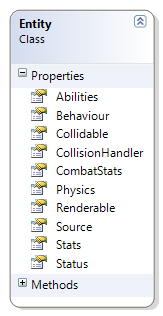
\includegraphics[scale=1]{graphics/entity}
    \caption{The components of the entity class}
    \label{fig:entity}
    \end{center}
\end{figure}

In short, everything you see on the screen, and quite a few things you don't
see, are implemented as Entities. Each entity is a container for different
components, which have clearly defined responsibilities. There are for 
instance:
\begin{itemize}
    \item Renderables (Used for showing things on screen)
    \item Behviours (Mostly used for AI, but also player control)
    \item Abilities (Which allow entities to interact with the game world)
    \item And many more, see the code for complete coverage.
\end{itemize}

This system allows us extreme flexibility in composing new features, and 
defining the world of our game. The primary guideline when developing this
system was modifiability, but there were some tradeoffs which had to be made.
The system is complex, and takes some time to understand. Complex code hinders
maintainability, which is closely related to modifiability. The endless 
possibilities of this system however far outweigh the downsides.

\begin{figure}
    \begin{center}
    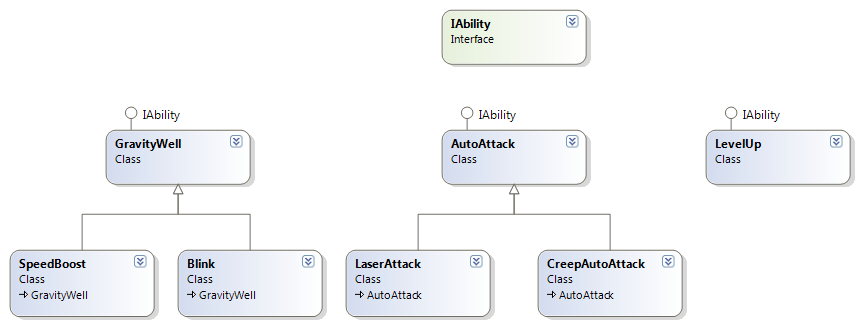
\includegraphics[width=\linewidth]{graphics/abilities}
    \caption{The Ability interface and implementing classes}
    \label{fig:abilities}
    \end{center}
\end{figure}

\begin{figure}
    \begin{center}
    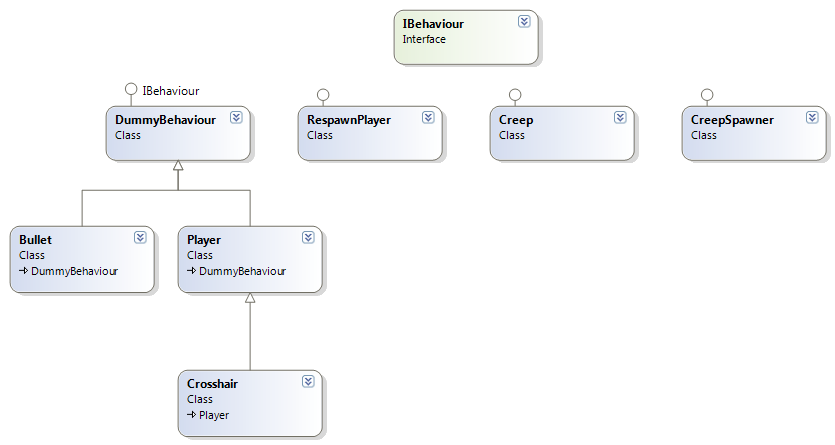
\includegraphics[width=\linewidth]{graphics/behaviours}
    \caption{The Behaviour interface and implementing classes}
    \label{fig:behaviours}
    \end{center}
\end{figure}

\begin{figure}
    \begin{center}
    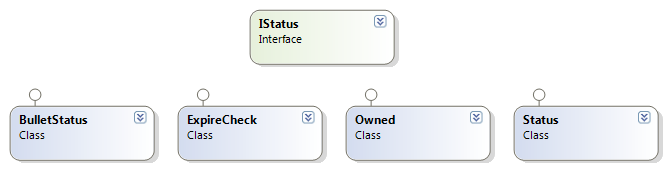
\includegraphics[width=\linewidth]{graphics/statuses}
    \caption{The Status interface and implementing classes}
    \label{fig:statuses}
    \end{center}
\end{figure}

To show just how flexible this system is, we will go through how two integral
features from the game were implemented using this system. They are the players
avatar in the game, and the entity which allows us to add hostiles to the 
world.

First the player. The important thing to note here is that the player is no
different from a hostile in the game. Sure they have more health and better
weapons (which are defined in data), but they follow the same rules as 
everybody. We do this by creating a custom behaviour for players which reads 
the state of the XBOX controller. This then directs the players entity, which
updates just as if it were any other creep.

The other example we wish to highlight is creep-spawners. These are responsible
for adding hostiles to the world. They are defined in data, and are invisible
to players (They could however be made visible, for instance creeps might be
deployed from a carrier). In terms of functionality they are as far removed 
from players as one could possibly come, but are still implemented using the
same base classes.  A creep-spawner is an entity whose only ability is to spawn
hostiles. They quite literally shoot hostiles into the world (using the exact
same code that players use to shoot their main cannon)

\subsection{progarkspill.GameStateStack}
A game usually has different phases, such as showing a splash-screen, menus and
obviously playing the game itself. We wanted these features, and asked 
ourselves how we could do this as elegantly as possible.  Our first solution
was to design an event-system which would queue state-changes and apply these
changes transparently to the states themselves. We decided early on however 
that we were over-engineering the problem, and changed this to a simple stack 
of states.

Each state has access to this stack, and can add or remove new states. We then
call methods on the top element of the stack, and everything works out neatly.
This solution introduces some coupling in the code, for instance any state 
which can lead into another state must know of the other state. An example is
the main menu which must know of the in-game state in order to start the game.
This would be avoided by using the aforementioned event-system, but we feel
our current system works well enough, and the downsides are small compared to
the extreme simplicity of this system. As the program starts we populate the
stack with the menu, and we quit the game when the stack is empty.

\subsection{progarkSpill.GameState}
This class represents the state of being in the playable portion of the game. 
It is a good place to start understanding the sequence of logic in the game.

The class is unfortunately very large, and has many responsibilities. For 
instance this is where we store the current level, it contains a list of all
players and hostiles, and also encodes the winning and losing conditions. It is
the closest we have come to a \emph{god-object}, so-named because it knows
everything and can do anything, which plagues many game architectures.

This is the one thing in our project which we are truly unhappy with, and the
first thing to be revised if we had more time to do it. There is not a single
redeeming feature to having a large monolithic class with such disparate
responsibilities, aside from the fact that it is an incredibly easy and quick
solution.

\subsection{progarkSpill.MenuState}
This is a group of classes which represents the different menus in the game.
While they are simple and powerful, we do wish we could make these more
data-driven, and perhaps a lot more pretty in terms of graphics.

Each class has two methods which implements most of the functionality of that
menu. A total of four menus were implemented, the main menu, two menus 
displayed  after winning or losing the game, and a pause-menu.

\subsection{progarkSpill.Controller}
This is a single class containing nothing but static methods and members. It
was created as a layer of abstraction above XNAs similar GamePad class, but
contains one more feature we needed for our game, namely tracking the time a
certain button was pressed. It would also be the place any other controller-
related features were added. This class resembles the \emph{Singleton-pattern}
closely, in that it provides global access and a single point of responsibility
for controllers. It is not implemented in the way that singletons usually are
however. We chose to use all static members, and drop the silly getInstance()-
interface one often sees in this pattern.

\subsection{progarkSpill.Renderer}
This subsystem is the only way to display graphics on the screen, and an
instance to it is passed around to nearly all portions of the code. It was
designed to be extendable and configurable in most ways, but we never needed
this extensibility. The renderer could, if needed, maintain internal lists of
all submitted render-jobs, reorder them for optimization, or share state 
between jobs for extensibility. We also planned to use Post-Processing effects,
but this feature was scrapped due to time-constraints.

What we wound up with is a class which can display graphics in many ways, and
which can be configured by the game through the IRenderable interface. Due to
some miscommunication in the start of the project the interface was not 
implemented as planned, but all the features we planned for (with the noted
exception of the effects) are still available.

\subsection{progarkSpill.ViewPort}
This is a class which handles transforms between the game's coordinate-system
and the screen. It was implemented to allow different screen-sizes (i.e. on
HD-Ready and Full-HD screens), and to allow us to think in terms of a natural
unit of measurement such as meters, instead of thinking in terms of pixels.